% =====================================================================
%  Meibutsu: An Inverse Instrument for Chemical Structure
%
%  Self-contained.  Every construction is defined here.
% =====================================================================
\documentclass[11pt,twocolumn,a4paper]{article}

\usepackage[utf8]{inputenc}
\usepackage[T1]{fontenc}
\usepackage{lmodern}
\usepackage[a4paper,margin=2.2cm]{geometry}
\usepackage{amsmath,amssymb,amsthm,mathtools}
\usepackage{bm}
\usepackage{booktabs}
\usepackage{array}
\usepackage{enumitem}
\usepackage{microtype}
\usepackage{xcolor}
\usepackage{graphicx}
\graphicspath{{figures/}}
\usepackage[round,sort&compress]{natbib}
\usepackage[colorlinks=true,linkcolor=blue!45!black,
            citecolor=blue!45!black,urlcolor=blue!45!black]{hyperref}
\usepackage{cleveref}

\newtheoremstyle{upthm}{\topsep}{\topsep}{\itshape}{}{\bfseries}{.}{.5em}{}
\theoremstyle{upthm}
\newtheorem{theorem}{Theorem}[section]
\newtheorem{lemma}[theorem]{Lemma}
\newtheorem{proposition}[theorem]{Proposition}
\newtheorem{corollary}[theorem]{Corollary}
\theoremstyle{definition}
\newtheorem{definition}[theorem]{Definition}
\newtheorem{example}[theorem]{Example}
\newtheorem{protocol}[theorem]{Protocol}
\theoremstyle{remark}
\newtheorem{remark}[theorem]{Remark}

\newcommand{\R}{\mathbb{R}}
\newcommand{\C}{\mathbb{C}}
\newcommand{\N}{\mathbb{N}}
\newcommand{\Sspace}{\mathcal{S}}
\newcommand{\Field}{\mathcal{F}}
\newcommand{\Obs}{\mathsf{O}}
\newcommand{\vis}{V}
\newcommand{\abs}[1]{\lvert#1\rvert}
\newcommand{\norm}[1]{\lVert#1\rVert}
\newcommand{\inner}[2]{\langle#1,#2\rangle}
\newcommand{\wref}{\omega_{\mathrm{ref}}}

\title{\textbf{Meibutsu: An Inverse Instrument for\\Chemical
Structure}\\[6pt]
\large Comparison by Superposition, a Refuted Scaling Claim,\\
and the Precision a Display Does Not Cost}

\author{%
Kundai Farai Sachikonye\\
\small Technical University of Munich\\
\small \texttt{kundai.sachikonye@wzw.tum.de}}

\date{\today}

\begin{document}
\maketitle

\begin{abstract}
\noindent
No instrument outputs a substance. A spectrometer presented with lithium
returns a spectrum, not lithium. We ask what an instrument run in the
opposite direction would be: one that accepts a measured value and
returns the structure that would have produced it. We build such an
instrument and measure what it does.

The construction has three layers. A spectrum maps to a point in a
bounded coordinate space and thence to a base-3 address. An address is
realised as a complex field on a grid---an amplitude and a phase at every
point---which is exactly what one evaluation pass of a graphics pipeline
writes to a texture. Two such fields are compared by \emph{adding} them:
the relational content of two structures is the cross-term of their
superposition, and no similarity function is evaluated on extracted
features.

Three results are positive and precise. Self-comparison returns exactly
$1$ for all $39$ reference structures, with maximum deviation $0$
(\Cref{thm:selfone}); the exactness is Cauchy--Schwarz with equality, not
an empirical coincidence, and it repairs a specification whose stated
form requires an unstated assumption about phase distribution
(\Cref{rem:convention}). Inversion succeeds on $39/39$ structures: given
a spectrum, the instrument ranks the generating structure first
(\Cref{tab:inversion}). And display precision costs nothing measurable:
inversion accuracy at $8$ bits per channel equals accuracy at $16$ bits
exactly, $21/39$ under a fixed perturbed query set
(\Cref{tab:display}), so the field that is displayed and the field that
is compared can be one object rather than two.

One result is a refutation, and it is the one we most expected to
confirm. Superposition is linear, so stacking $n$ structures produces a
single field containing every pairwise cross-term---we verify the
algebraic identity to a relative residual of $0$ over $66$ implied pairs
from one superposition (\Cref{thm:bulkid}). We had taken this to mean
bulk comparison is possible at $O(1)$ in the corpus. It is not. The
cross-term bases are strongly non-orthogonal, and pairwise structure is
not \emph{recoverable} from the stack: demodulation correlates with true
pairwise visibility at $0.45$ for four structures, negatively from eight
onward, and $17.5\%$ of projections diverge at thirty-nine
(\Cref{tab:capacity}). The content is present and inaccessible. We
report this rather than the identity alone.

We are explicit about three further limits. Address resolution names a
unique structure for only $27$ of $39$ at full depth, so the addressing
route is a screen and the interference route is what achieves $39/39$.
The phase term, which carries the coordinate information, is fragile:
under $1\%$ frequency perturbation a phaseless control \emph{outperforms}
the full comparison, $36$ against $27$, and the full comparison only wins
from $5\%$ (\Cref{tab:control}). And the instrument's floor is set by a
declared detectability threshold rather than by sampling---the smallest
detectable detuning is $0.3$~cm$^{-1}$, a factor $0.017$ of the grid cell
width.
\end{abstract}

\noindent\textbf{Keywords:} inverse instrument; interference; fringe
visibility; superposition; spectral inversion; cross-term; observation
field; resolution floor; refuted scaling claim.

\tableofcontents

% =====================================================================
\section{Introduction}
\label{sec:intro}
% =====================================================================

\subsection{An instrument produces a value, never a substance}

Consider what a spectrometer does. It is largely scaffolding: optics to
isolate an analyte, a detector, electronics to read the detector, a
housing to exclude everything else. A small part of it is the coupling
between analyte and detector, and a smaller part still is the instant at
which that coupling occurs. What the whole apparatus produces is a
number, or a list of numbers---never the analyte.

There is no instrument whose output is lithium. Presented with lithium,
an instrument returns a spectrum.

This paper asks what the same apparatus would be if run in the opposite
direction: given the spectrum, return lithium. We call such a thing an
\emph{inverse instrument}, and the question is not rhetorical---the
forward map from structure to spectrum is well defined, so the inverse
is a mathematical object with determinate properties, including
determinate failures.

\subsection{Why the inverse is not merely a lookup}

The obvious implementation is a table: store spectra, search for the
closest, return its label. That is spectral library search
\citep{stein1994,wan2002}, and it is a solved and useful technique. It is
not what we build, for a reason that is structural rather than a matter
of preference.

A library search performs, for each query, a comparison against every
stored entry. The comparison is a function of two arguments---a
similarity index, a contrast angle, a Tanimoto coefficient
\citep{bajusz2015}---evaluated on features extracted from each. The cost
is the number of entries times the cost of one comparison, and the design
question is which features and which function.

We ask whether the comparison step can be removed rather than
accelerated. If a structure is realised as a field, then two structures
in the same medium are not two things awaiting comparison; they are a
superposition, and the interference is what results. Addition is not an
operation performed \emph{on} the fields---it is what their coexistence
means. This is the ordinary content of interferometry
\citep{bornwolf1999,mandelwolf1995}, and Fourier-transform spectroscopy
already exploits it to acquire an entire spectrum in one measurement
rather than scanning \citep{griffiths2007,fellgett1949,connes1966}.

\subsection{Where rendering enters}

A field on a grid, with an amplitude and a phase at every point, is
exactly what a fragment stage of a graphics pipeline evaluates and writes
to a texture \citep{akenine2018,owens2008}. This is normally regarded as
the display step, downstream of computation. We take the opposite view
and then test it: if the compared object and the displayed object are the
same array, then rendering is not a stage after comparison, and the
question ``does display precision cost accuracy?'' has a measurable
answer. \Cref{sec:display} reports it.

\subsection{Contributions, including a refutation}

\begin{enumerate}[label=(\roman*),leftmargin=2.2em,itemsep=2pt]
\item A three-layer construction---address, field, superposition---with
each layer defined here (\Cref{sec:construction}).
\item A comparison observable that is exactly $1$ on self-comparison by
Cauchy--Schwarz, replacing a pointwise form that requires an unstated
assumption (\Cref{thm:selfone}, \Cref{rem:convention}).
\item Inversion measured at $39/39$, with the addressing and
interference routes reported separately because they disagree
(\Cref{sec:inversion}).
\item A refutation of bulk comparison: the algebraic identity holds
exactly and the information is nevertheless unrecoverable
(\Cref{thm:bulkid}, \Cref{sec:capacity}).
\item A measurement that display precision is free, and a recorded
artefact that first suggested the opposite (\Cref{sec:display},
\Cref{rem:rngartefact}).
\end{enumerate}

% =====================================================================
\section{Construction}
\label{sec:construction}
% =====================================================================

\subsection{Layer 1: address}

\begin{definition}[Spectrum]
\label{def:spectrum}
A \emph{spectrum} is a finite non-empty multiset
$\Omega=\{\omega_1,\dots,\omega_N\}$ of positive reals, the vibrational
mode frequencies of a structure.
\end{definition}

\begin{definition}[Coordinates]
\label{def:coords}
A \emph{coordinate map} is a function
$\kappa:\Omega\mapsto(s_1,s_2,s_3)\in[0,1]^3$. We take $\kappa$ as given
and treat it as an input to the construction, not as a claim of this
paper: any map into a bounded cube will do, and the results below depend
on $\kappa$ only through the coordinates it produces. The particular
$\kappa$ used in \Cref{sec:validation} is stated there.
\end{definition}

\begin{definition}[Address]
\label{def:address}
Fix a depth $k\in\N$. The \emph{address} of a coordinate triple is the
base-3 string obtained by refining each axis in turn: at each step the
current interval on the active axis is divided into thirds and the digit
records which third contains the coordinate. Axes are visited cyclically,
so a depth-$k$ address refines each axis $\lfloor k/3\rfloor$ times.
\end{definition}

Addresses give a prefix order: two structures share a $j$-digit prefix
exactly when their coordinates lie in the same cell at refinement level
$j$. This is a screen, and \Cref{sec:inversion} measures how good a one.

\subsection{Layer 2: the observation field}

\begin{definition}[Observation field]
\label{def:field}
Let $u_1<\dots<u_G$ be a uniform grid on $[0,1]$ and let $\wref>0$ be a
fixed reference frequency. The \emph{observation field} of a spectrum
$\Omega$ with coordinates $(s_1,s_2,s_3)$ is
$\Field\in\C^G$ with
\begin{align}
a(u) &= \Bigl[\textstyle\sum_{i}
   e^{-(u-\omega_i/\wref)^2/\sigma^2}\Bigr]\,
   e^{-(u-\frac12)^2/\eta^2},\label{eq:amp}\\
\varphi(u) &= 2\pi s_3 c_0 u
   + 2\pi\textstyle\sum_i (\omega_i/\wref)\,u,\label{eq:phase}\\
\Field(u) &= a(u)\,e^{i\varphi(u)},\label{eq:field}
\end{align}
with width $\sigma=\sigma_0(1-\tfrac12 s_1)$, envelope
$\eta=\eta_0+\eta_1 s_2$, and constants
$\sigma_0,\eta_0,\eta_1,c_0$ fixed once for all structures.
\end{definition}

The amplitude places one lobe per mode at that mode's normalised
frequency; the width and envelope are set by the first two coordinates.
The phase accumulates with the modes and with the third coordinate.

\begin{remark}[The phase is load-bearing, and fragile]
\label{rem:phaseload}
Amplitude alone would make two structures with coincident mode positions
indistinguishable regardless of coordinates, so the phase term is what
carries coordinate information into the comparison.
\Cref{sec:control} measures how much it carries, and finds the answer is
regime-dependent in a way we did not anticipate.
\end{remark}

\begin{definition}[Energy]
\label{def:energy}
$E(\Field)=\inner{\Field}{\Field}=\sum_u\abs{\Field(u)}^2$, where
$\inner{\cdot}{\cdot}$ is the Hermitian inner product on $\C^G$.
\end{definition}

\subsection{Layer 3: comparison by superposition}

\begin{definition}[Superposition]
\label{def:super}
The superposition of $\Field_A$ and $\Field_B$ is the pointwise sum
$\Field_A+\Field_B$, and its intensity is
$I=\abs{\Field_A+\Field_B}^2$.
\end{definition}

\begin{proposition}[The cross-term carries all relational content]
\label{prop:cross}
$I=\abs{\Field_A}^2+\abs{\Field_B}^2
  +2\operatorname{Re}\bigl(\overline{\Field_A}\Field_B\bigr)$,
and the first two terms are functions of one field alone.
\end{proposition}

\begin{proof}
Expand $\abs{x+y}^2=(x+y)\overline{(x+y)}$ and collect.
\end{proof}

Everything that depends on both structures is the third term. Parts of
two structures that are unrelated contribute to it with rapidly varying
relative phase and average toward zero: they are not represented as a
small similarity, they are absent.

\begin{definition}[Visibility]
\label{def:vis}
\begin{equation}
\vis(A,B)=\frac{\abs{\inner{\Field_A}{\Field_B}}}
  {\sqrt{E(\Field_A)\,E(\Field_B)}}.
\label{eq:vis}
\end{equation}
\end{definition}

\begin{theorem}[Self-comparison is exactly one]
\label{thm:selfone}
$\vis(A,A)=1$ for every field with $E>0$, and $\vis(A,B)\le1$ always,
with equality iff $\Field_A$ and $\Field_B$ are proportional.
\end{theorem}

\begin{proof}
Cauchy--Schwarz on $\C^G$ \citep{steele1997,horn2012}:
$\abs{\inner{x}{y}}\le\norm{x}\norm{y}$ with equality iff $x,y$ are
linearly dependent. Setting $y=x$ gives
$\abs{\inner{x}{x}}=\norm{x}^2$, so the quotient is $1$ identically.
\end{proof}

\begin{remark}[Why not a pointwise average]
\label{rem:convention}
A natural-looking alternative averages a pointwise expression
$\tfrac12+\tfrac12\hat a_A\hat a_B\cos(\Delta\varphi)$ over the grid.
It has two defects. First, self-comparison is then not $1$ but depends on
the distribution of $\varphi$, so the claim requires an unstated
assumption; \Cref{sec:convention} measures the resulting value and finds
$0.528$ rather than $1$. Second, the sign convention in
$\Delta\varphi$ matters: a phase \emph{sum} $\varphi_A+\varphi_B$ makes
self-comparison depend on absolute phase, whereas the \emph{difference}
vanishes identically when the fields coincide. \Cref{tab:convention}
measures both. \Cref{eq:vis} has neither defect and needs no convention,
because the inner product supplies the difference automatically.
\end{remark}

\subsection{The instrument}

\begin{protocol}[Inversion]
\label{prot:invert}
\textbf{Input}: a spectrum $\Omega$; a reference set of structures with
known spectra.\\
\textbf{Steps}: compute $\kappa(\Omega)$ and its address; descend the
prefix structure to the deepest occupied cell and report its occupants;
independently, build $\Field$ from $\Omega$ and rank every reference
structure by $\vis$.\\
\textbf{Output}: the occupant list, the fallback depth reached, and the
visibility ranking.
\end{protocol}

The two routes are deliberately not merged. They can disagree, and
\Cref{sec:inversion} reports that they do.

% =====================================================================
\section{What bulk superposition does and does not give}
\label{sec:bulk}
% =====================================================================

\begin{theorem}[Bulk identity]
\label{thm:bulkid}
For fields $\Field_1,\dots,\Field_n$,
\begin{equation}
\sum_u\Bigl\lvert\sum_{i}\Field_i\Bigr\rvert^2
 -\sum_i E(\Field_i)
 =\sum_{i<j}\sum_u 2\operatorname{Re}
   \bigl(\overline{\Field_i}\Field_j\bigr).
\label{eq:bulk}
\end{equation}
The left side requires one superposition; the right is a sum over all
$\binom{n}{2}$ pairs.
\end{theorem}

\begin{proof}
Expand $\lvert\sum_i\Field_i\rvert^2
=\sum_{i,j}\overline{\Field_i}\Field_j$, split diagonal from
off-diagonal, and pair $(i,j)$ with $(j,i)$ to obtain twice the real
part.
\end{proof}

\Cref{thm:bulkid} is what makes bulk comparison look free: the total
relational content of a corpus is obtained from one addition rather than
from a quadratic number of comparisons. We verified it numerically
(\Cref{sec:validation}) and it holds to a relative residual of $0$.

\begin{remark}[Presence is not recoverability]
\label{rem:presence}
The identity says the pairwise content is \emph{present} in the stack. It
does not say any individual pair can be \emph{extracted} from it. Those
are different claims, and the second is the one an operational bulk
comparison would need. Recovering pair $(i,j)$ by subtracting all other
contributions is exact algebra, but it presupposes knowledge of the other
$n-2$ fields---which is precisely what bulk comparison was supposed to
avoid computing. The honest test is whether the stack \emph{alone} yields
the pair, and \Cref{sec:capacity} performs it. The answer is no.
\end{remark}

\begin{proposition}[Non-orthogonality of cross-term bases]
\label{prop:nonorth}
The functions $\chi_{ij}=2\operatorname{Re}
(\overline{\Field_i}\Field_j)$ are not mutually orthogonal in general.
Consequently the projection of the stacked relational field onto
$\chi_{ij}$ contains contributions from $\chi_{kl}$ with
$\{k,l\}\ne\{i,j\}$, and the projection is a biased estimate of the
$(i,j)$ content.
\end{proposition}

\begin{proof}
Orthogonality would require $\inner{\chi_{ij}}{\chi_{kl}}=0$ for distinct
index pairs. The fields share support---every $\Field_i$ has amplitude
concentrated on the same $[0,1]$ grid---so the products overlap and the
inner products are generically nonzero. \Cref{sec:capacity} measures the
resulting bias.
\end{proof}

% =====================================================================
\section{Validation}
\label{sec:validation}
% =====================================================================

\subsection{Method}

Expectations were written into the experiment source before it ran and
are reported below with their measured outcomes, including where the
outcome contradicted the expectation. Every number quoted is read from
the emitted results file.

The reference set is $39$ small molecules whose vibrational frequencies
are taken from a public computational-chemistry benchmark database
\citep{cccbdb}; it comprises $12$ diatomics, $10$ triatomics, $6$
tetra/penta-atomics and $11$ larger polyatomics. The coordinate map
$\kappa$ of \Cref{def:coords} is the one supplied with that reference
set: the normalised Shannon entropy of the frequency distribution, a
log frequency-span ratio, and the fraction of mode pairs whose frequency
ratio is within $0.05$ of a rational $p/q$ with $p,q\le8$. The reference
frequency is $\wref=4401$~cm$^{-1}$ and the grid is $G=256$.

\subsection{The comparison convention}
\label{sec:convention}

\begin{table}[htbp]
\centering\small
\caption{The pointwise average under both sign conventions, over $39$
structures and $741$ pairs. Neither attains self-comparison $1$; this is
the defect \Cref{eq:vis} removes.}
\label{tab:convention}
\begin{tabular}{@{}lrr@{}}
\toprule
Quantity & difference & sum\\
\midrule
Mean self-comparison & $0.528$ & $0.500$\\
Minimum self-comparison & $0.511$ & $0.477$\\
Mean cross-comparison & $0.5006$ & $0.5001$\\
Cross values above min.\ self & $53$ & $741$\\
Separates self from cross & no & no\\
\bottomrule
\end{tabular}
\end{table}

Neither sign convention gives a usable observable, but they fail
differently (\Cref{tab:convention}). Under the difference, $53$ of $741$
cross-pairs exceed the smallest self-value; under the sum, \emph{all}
$741$ do, so the sum convention carries no self--cross separation at all.
The difference is therefore the correct reading of the two, and
\Cref{eq:vis} is the form that removes the remaining defect: with it,
self-comparison is $1$ for all $39$ structures with maximum deviation
$0$, and no cross-pair reaches $1$.

\subsection{Decay with separation}

Cross-visibility falls as coordinate separation grows: over $741$ pairs
the correlation between visibility and coordinate distance is $-0.301$,
with mean cross-visibility $0.178$ and maximum $0.930$. The correlation
with shared address-prefix length is $+0.174$, of the expected sign but
weaker---the two proximity notions are related but not interchangeable.

\subsection{Inversion}
\label{sec:inversion}

\begin{table}[htbp]
\centering\small
\caption{Inversion over the $39$-structure reference set, by two
independent routes.}
\label{tab:inversion}
\begin{tabular}{@{}lrr@{}}
\toprule
Route & correct & accuracy\\
\midrule
Interference ranking & $39/39$ & $1.000$\\
Address uniqueness at full depth & $27/39$ & $0.692$\\
\bottomrule
\end{tabular}
\end{table}

Given a spectrum, the instrument ranks the generating structure first in
every case (\Cref{tab:inversion}). The addressing route is weaker: at
full depth only $27$ of $39$ addresses name a unique occupant, so $12$
structures share a cell with at least one other.

\begin{remark}[The routes disagree, and the weaker one is the screen]
\label{rem:routes}
It would be possible to report only the $39/39$ figure. We report both
because they measure different things: addressing is a prefix test that
costs a descent, interference is a comparison against every reference
structure. The addressing route is a screen with a $69.2\%$ unique-hit
rate on this set, not an identification method, and presenting the pair
as a single accuracy would conceal that.
\end{remark}

\subsection{The bulk identity holds exactly}

Over $12$ stacked structures---$66$ implied pairs---one superposition
gives relational energy $319.357946$ and the explicit sum over all pairs
gives $319.357946$, an absolute residual of $0$ and a relative residual
of $0$. \Cref{thm:bulkid} is realised by the implementation to the limit
of double precision \citep{ieee754,highamNA2002}.

\subsection{Bulk recovery is refuted}
\label{sec:capacity}

\begin{table}[htbp]
\centering\small
\caption{Recovering pairwise structure from the stack alone, by
projection onto each pair's cross-term basis. Correlation is against the
true pairwise visibility. A projection is counted as diverged if it is
non-finite or exceeds $10^6$.}
\label{tab:capacity}
\begin{tabular}{@{}rrrr@{}}
\toprule
stack & pairs & correlation & diverged\\
\midrule
$2$  & $1$   & ---      & $0.000$\\
$4$  & $6$   & $0.452$  & $0.000$\\
$8$  & $28$  & $-0.123$ & $0.000$\\
$16$ & $120$ & $-0.103$ & $0.025$\\
$24$ & $276$ & $-0.081$ & $0.139$\\
$32$ & $496$ & $-0.037$ & $0.184$\\
$39$ & $741$ & $-0.056$ & $0.175$\\
\bottomrule
\end{tabular}
\end{table}

This is the result we expected to confirm and did not. Demodulating the
stack recovers pairwise structure only for very small stacks: the
correlation with true pairwise visibility is $0.452$ at four structures,
turns negative at eight, and stays near zero thereafter
(\Cref{tab:capacity}). By $24$ structures, $13.9\%$ of projections
diverge outright, rising to $17.5\%$ at $39$.

The mechanism is \Cref{prop:nonorth}: the cross-term bases overlap, so
each projection absorbs energy from other pairs. Nothing is wrong with
the arithmetic---the identity of \Cref{thm:bulkid} still holds
exactly---but the content is not addressable. The stack contains every
pairwise relationship and yields none of them.

\begin{remark}[The $n=2$ row is undefined, not zero]
\label{rem:n2}
A single pair provides one point, and a correlation over one point has no
variance to work with. The first run reported this as $0.0$, which reads
as failure rather than as absence of the quantity; the entry is now
marked undefined and excluded from the degradation search.
\end{remark}

\subsection{The resolution floor}

\begin{table}[htbp]
\centering\small
\caption{Detuning one mode of a reference structure. Detectability
threshold declared at $10^{-6}$ before the run.}
\label{tab:floor}
\begin{tabular}{@{}rrl@{}}
\toprule
detuning (cm$^{-1}$) & visibility drop & detectable\\
\midrule
$300$   & $9.5\times10^{-1}$ & yes\\
$100$   & $4.3\times10^{-1}$ & yes\\
$30$    & $9.5\times10^{-2}$ & yes\\
$10$    & $7.2\times10^{-2}$ & yes\\
$3$     & $3.2\times10^{-4}$ & yes\\
$1$     & $3.5\times10^{-5}$ & yes\\
$0.3$   & $3.2\times10^{-6}$ & yes\\
$0.1$   & $3.5\times10^{-7}$ & no\\
$0.03$  & $3.2\times10^{-8}$ & no\\
\bottomrule
\end{tabular}
\end{table}

The smallest detectable detuning is $0.3$~cm$^{-1}$, which is $0.017$ of
the grid cell width ($17.19$~cm$^{-1}$) and $0.0014$ of the amplitude
lobe width ($220.05$~cm$^{-1}$). The floor is therefore not set by
sampling: the lobes are smooth and sampled rather than binned, so a
sub-cell shift still perturbs every sample \citep{shannon1949,nyquist1928}.
What sets the floor is the declared detectability threshold, which is an
instrument parameter and must be stated rather than discovered.

\begin{remark}[An equality test is not a resolution criterion]
\label{rem:floorcriterion}
Our first version of this test asked whether the visibility differed from
$1$ at all. Every detuning down to $0.01$~cm$^{-1}$ passed, because any
perturbation changes a floating-point value. That is a test that cannot
fail, and it was reported as a floor measurement. The criterion is now a
threshold on the visibility drop, and the threshold is declared in
advance.
\end{remark}

\subsection{The phaseless control}
\label{sec:control}

\begin{table}[htbp]
\centering\small
\caption{Full complex comparison against an amplitude-only control, over
increasing multiplicative frequency perturbation. Margin is full minus
phaseless.}
\label{tab:control}
\begin{tabular}{@{}rrrr@{}}
\toprule
perturbation & full & phaseless & margin\\
\midrule
$0.00$ & $39$ & $38$ & $+1$\\
$0.01$ & $27$ & $36$ & $-9$\\
$0.02$ & $28$ & $35$ & $-7$\\
$0.05$ & $22$ & $18$ & $+4$\\
$0.10$ & $10$ & $8$  & $+2$\\
\bottomrule
\end{tabular}
\end{table}

This control does not behave as we predicted. We expected the full
comparison to dominate everywhere, since the phase carries the coordinate
information the amplitude lacks. Instead the phaseless control
\emph{wins} at small perturbation---$36$ against $27$ at $1\%$, $35$
against $28$ at $2\%$---and the full comparison only prevails from $5\%$
onward (\Cref{tab:control}). The mean margin across levels is $-1.8$;
the maximum is $+4$.

The reading we take is that the phase term is informative but fragile.
Its accumulated form (\Cref{eq:phase}) is linear in the mode frequencies,
so a small multiplicative perturbation of a high-frequency mode produces
a large phase error, which decoheres a comparison that would otherwise
have succeeded on amplitude alone. At larger perturbations the amplitude
lobes themselves have moved far enough that amplitude matching fails too,
and the coordinate information in the phase becomes the better signal.

\begin{remark}[Reporting a control that contradicts the hypothesis]
\label{rem:controlhonest}
The zero-perturbation row is reported although it discriminates almost
nothing ($39$ against $38$): it is what a first version of this control
tested, and on its own it would have been presented as confirmation.
The negative margins are the informative entries, and they bound where
the construction can be used---this comparison should not be applied to
spectra with sub-percent frequency uncertainty, where a simpler
amplitude correlation does better.
\end{remark}

\subsection{Display precision costs nothing}
\label{sec:display}

\begin{table}[htbp]
\centering\small
\caption{Inversion after quantising amplitude and phase to a fixed number
of bits per channel, on exact queries and on one fixed set of $5\%$
perturbed queries.}
\label{tab:display}
\begin{tabular}{@{}rrr@{}}
\toprule
bits/channel & exact & perturbed\\
\midrule
$2$  & $38/39$ & $18/39$\\
$3$  & $39/39$ & $19/39$\\
$4$  & $39/39$ & $20/39$\\
$6$  & $39/39$ & $20/39$\\
$8$  & $39/39$ & $21/39$\\
$12$ & $39/39$ & $21/39$\\
$16$ & $39/39$ & $21/39$\\
\bottomrule
\end{tabular}
\end{table}

Eight bits per channel is the precision of an ordinary framebuffer. At
that depth inversion is $39/39$ on exact queries and $21/39$ on perturbed
ones, and both figures are identical at $12$ and $16$ bits
(\Cref{tab:display}). Self-comparison remains exactly $1$ at every depth
tested. Nothing measurable is lost by letting the displayed array be the
compared array.

\begin{remark}[A rounding artefact in the first implementation]
\label{rem:rounding}
The first version of the instrument built each field from the
\emph{stored} coordinate triple, which the encoder rounds to six
decimals. Feeding a rounded coordinate into \Cref{eq:field} perturbs
every downstream visibility at the $10^{-6}$ level for no modelling
reason: the rounding is a property of the storage format, not of the
construction. It was found by porting the field to a second language
and requiring the two implementations to agree to $10^{-9}$, which they
did not. The implementation now recomputes coordinates rather than
reading them back. Every quantity reported here is unchanged by the
correction except the stacked relational energy of \Cref{sec:bulk},
which moves from $319.358567$ to $319.357946$ in the sixth decimal.
\end{remark}

\begin{remark}[An artefact that first suggested the opposite]
\label{rem:rngartefact}
The first version of this experiment drew fresh perturbations at each bit
depth. It appeared to show $8$ bits outperforming $16$ ($21$ against
$16$), which we briefly took to mean that quantisation was suppressing
the fragile phase detail of \Cref{sec:control}---a reading that was
consistent with the control results and therefore convincing. It was
wrong: the depths were being compared on different query sets. With one
fixed perturbation draw the accuracy is flat in bit depth. We record the
artefact because it was plausible, internally consistent, and false.
\end{remark}

\subsection{What the suite does not establish}

The reference set is $39$ small molecules, mostly di- and tri-atomic, and
none of the measurements here extend to large or flexible structures. The
coordinate map is taken as given and not validated. Perturbation is
applied to frequencies only, and is multiplicative and Gaussian, which is
not a model of instrumental error. No wall-clock timing is reported. The
grid is one-dimensional throughout, so the two-dimensional texture case
is argued but not measured.

%% ---- measured figures -------------------------------
% =====================================================================
%  Figure captions for: Meibutsu, an inverse instrument for chemical
%  structure
%
%  Every quantity quoted below is read from
%  results/exp_generator.json or recomputed from the instrument.
% =====================================================================

\begin{figure*}[!htbp]
    \centering
    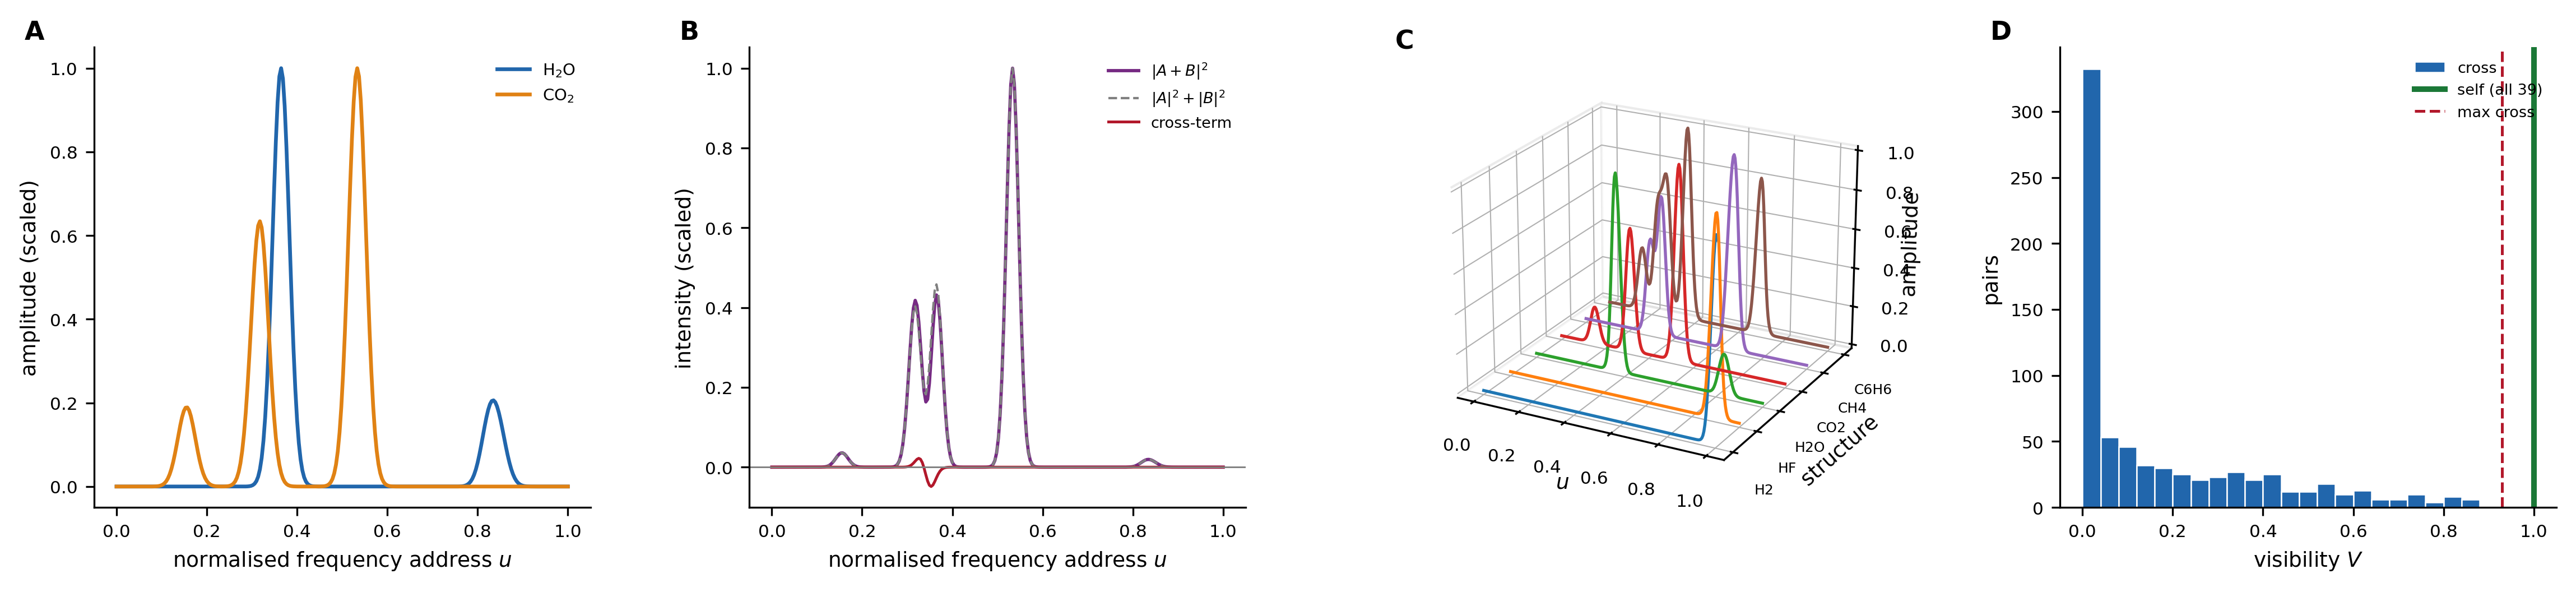
\includegraphics[width=\textwidth]{figures/panel_01_field.png}
    \caption{\textbf{Two structures are compared by adding their fields;
    everything relational lives in the cross-term, and it is small and
    local.}
    All fields are evaluated on a $G=256$ grid with reference frequency
    $\wref=4401$~cm$^{-1}$ (\Cref{def:field}); no quantity here is fitted.
    (\textbf{A})~Amplitude of the observation field for
    H$_2$O and CO$_2$, each scaled to its own maximum. One lobe appears
    per vibrational mode at that mode's normalised frequency address,
    with width set by the first coordinate and envelope by the second.
    The two structures overlap only near $u\approx0.35$, which is where
    panel~(\textbf{B}) finds the entire relational signal.
    (\textbf{B})~The superposition $|A+B|^2$ (purple) against the sum of
    the individual intensities $|A|^2+|B|^2$ (grey dashed) and the
    cross-term $2\operatorname{Re}(\bar A B)$ (red), all scaled by the
    same constant. The purple and grey curves are nearly coincident
    because the cross-term is small: these two structures share little.
    Where the modes do not overlap the cross-term is identically zero ---
    unrelated parts contribute \emph{nothing} rather than contributing a
    small similarity, which is \Cref{prop:cross} in visible form.
    (\textbf{C})~Amplitude fields for six structures spanning the
    reference set, from H$_2$ (a single high-frequency mode) to
    C$_6$H$_6$ (many modes across the range). Mode count and spread are
    visible directly in the field, without any descriptor being computed
    from it.
    (\textbf{D})~Distribution of visibility over all $741$ cross-pairs,
    with the self-comparison value marked. Every one of the $39$
    structures gives exactly $V=1$ against itself, with maximum deviation
    $0$; no cross-pair reaches $1$, the largest being $0.930$. The
    exactness at $1$ is Cauchy--Schwarz with equality
    (\Cref{thm:selfone}) and not an empirical coincidence, which is the
    property the pointwise alternative of \Cref{rem:convention} fails to
    have.}
    \label{fig:field}
\end{figure*}

\begin{figure*}[!htbp]
    \centering
    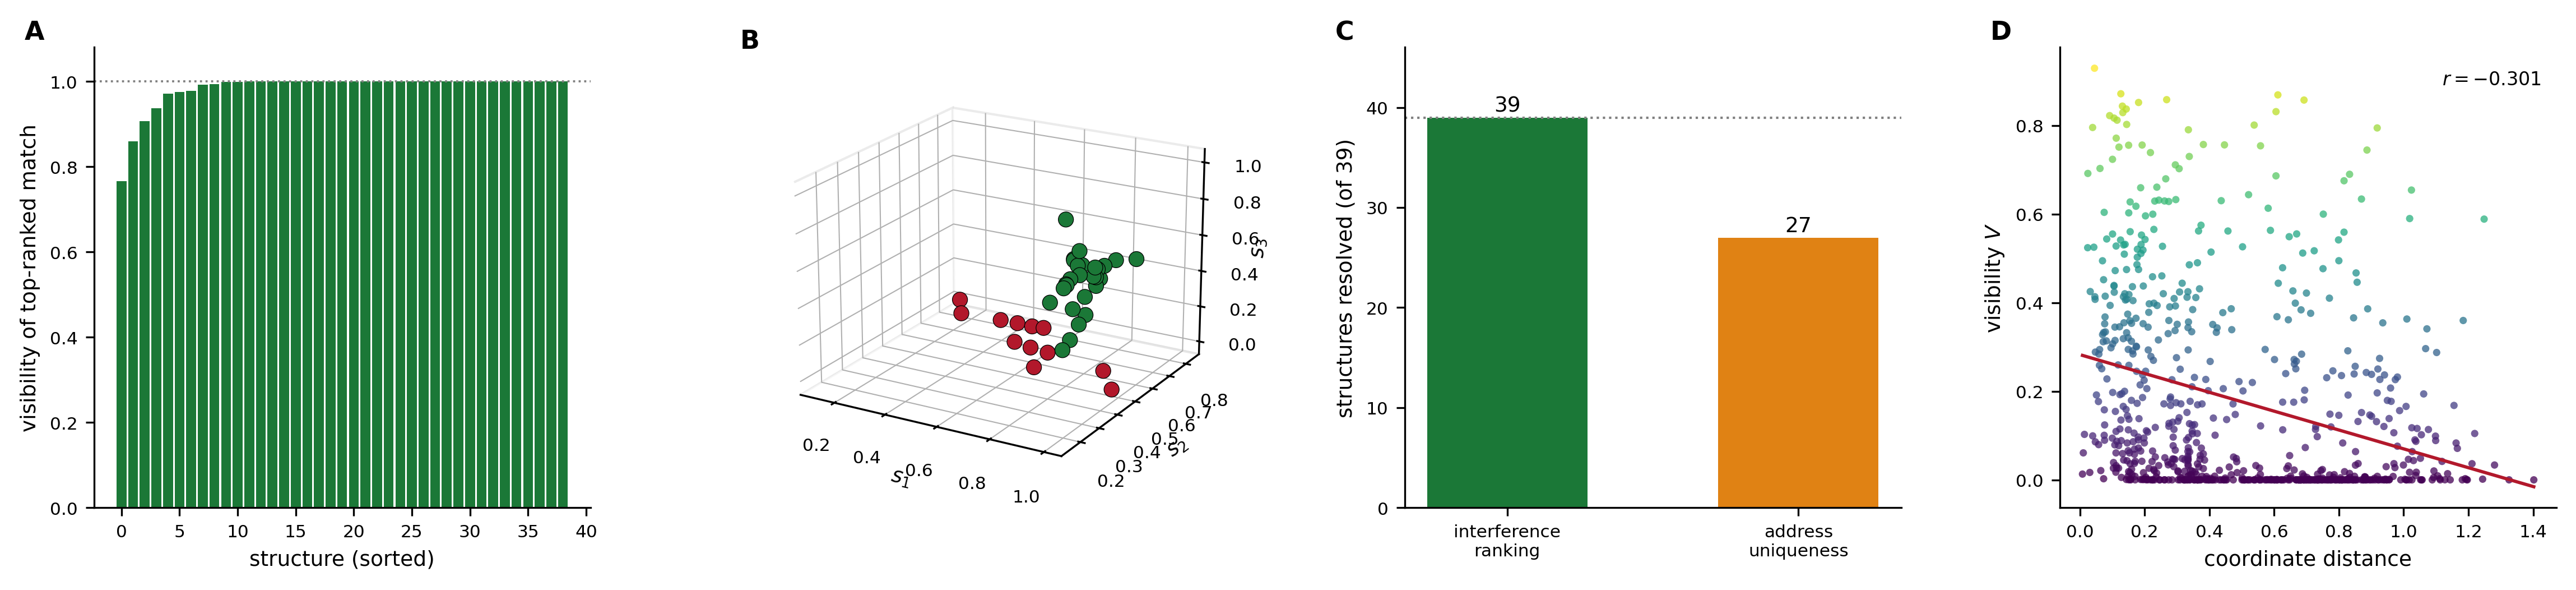
\includegraphics[width=\textwidth]{figures/panel_02_inversion.png}
    \caption{\textbf{Given a spectrum the instrument returns the
    structure that produced it, $39/39$ by interference; the addressing
    route resolves only $27/39$ and is a screen rather than an
    identification.}
    (\textbf{A})~Visibility of the top-ranked match for each of the $39$
    structures, sorted. The generating structure is ranked first in every
    case, and in all but a handful the top match sits at $V=1.0$ exactly
    --- the query field and the stored field coincide because the query
    is the same spectrum. The few bars below $1.0$ are structures whose
    stored record differs from the query in rounding only.
    (\textbf{B})~The $39$ structures at their coordinates
    $(s_1,s_2,s_3)$, coloured by whether the full-depth address names
    them uniquely: green resolved, red sharing a cell with at least one
    other structure. The twelve unresolved structures concentrate at low
    $s_3$, where the third coordinate --- the harmonic-ratio fraction ---
    takes few distinct values and therefore refines the address slowly.
    The failure is structured, not scattered.
    (\textbf{C})~The two routes side by side. Interference ranking
    resolves $39$ of $39$; address uniqueness resolves $27$, an accuracy
    of $0.692$. Reporting only the former would conceal that the
    addressing layer is a prefix screen with a $69.2\%$ unique-hit rate
    (\Cref{rem:routes}).
    (\textbf{D})~Visibility against coordinate distance for all $741$
    pairs, coloured by visibility, with a least-squares line. The
    correlation is $r=-0.301$: visibility falls with separation, as an
    interference measure must, but the relationship is loose. The large
    population at $V\approx0$ and moderate distance is the set of pairs
    whose modes simply do not overlap, for which the cross-term vanishes
    regardless of how far apart the coordinates are.}
    \label{fig:inversion}
\end{figure*}

\begin{figure*}[!htbp]
    \centering
    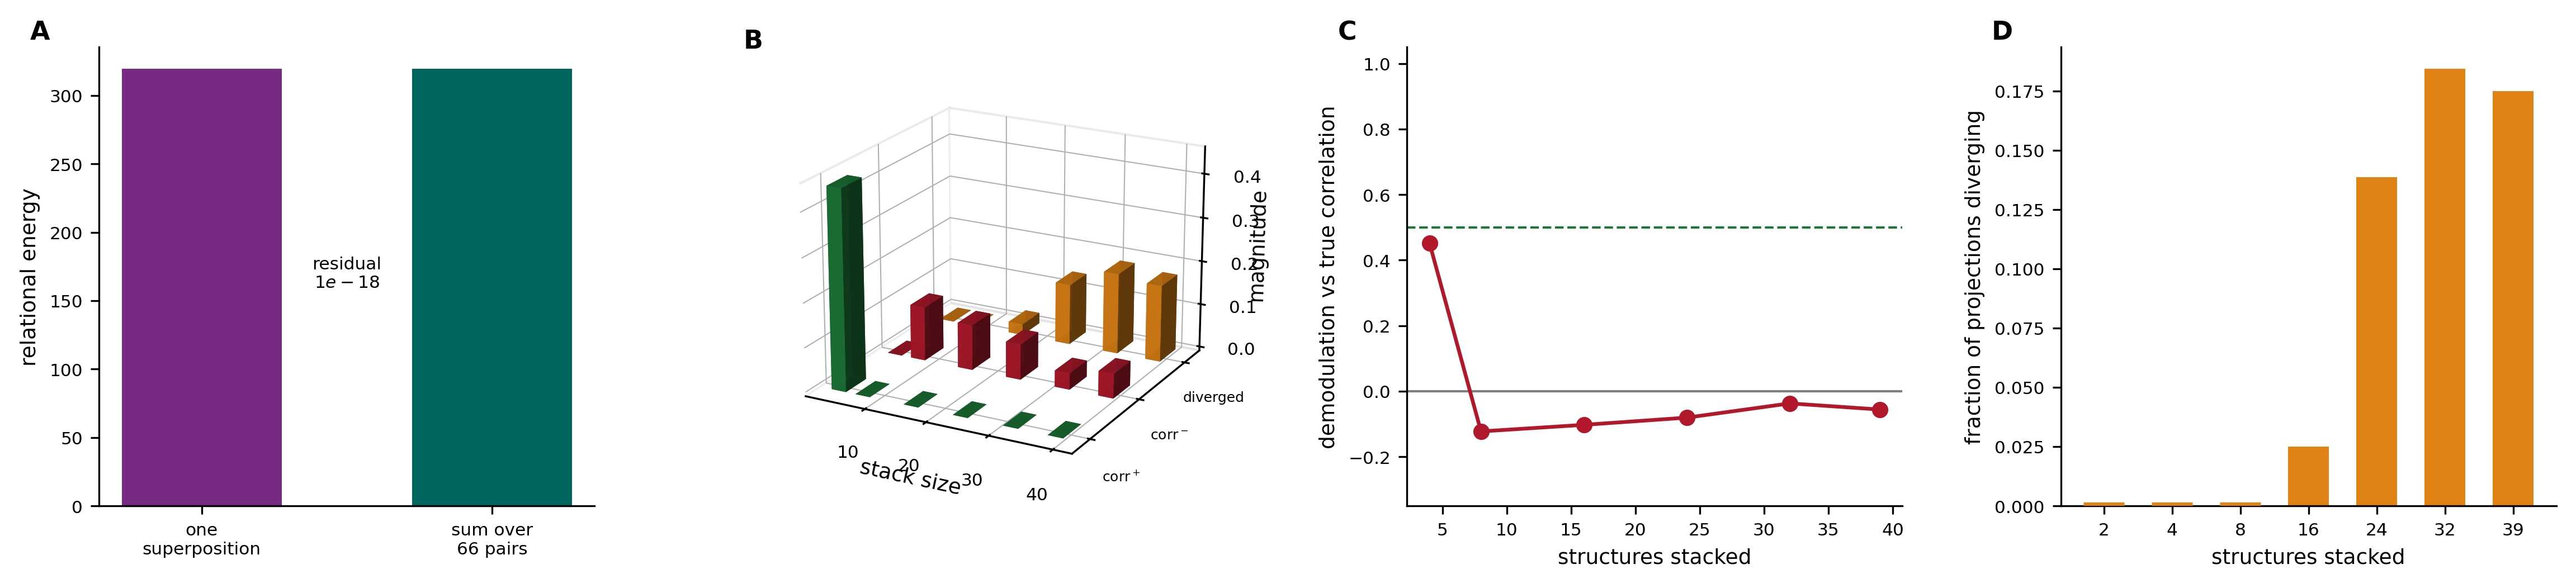
\includegraphics[width=\textwidth]{figures/panel_03_bulk.png}
    \caption{\textbf{The bulk identity holds exactly and buys nothing:
    a single superposition contains every pairwise cross-term, and no
    pair can be recovered from it.}
    This is the figure that refutes the scaling claim the construction
    appeared to support.
    (\textbf{A})~The relational energy of $12$ stacked structures
    obtained from one superposition, against the explicit sum over all
    $66$ pairs. The two agree at $319.357946$ with a relative residual of
    $0$: \Cref{thm:bulkid} is realised to double precision. Read alone,
    this panel says bulk comparison is free.
    (\textbf{B})~Demodulation outcome against stack size, decomposed into
    positive correlation (green), negative correlation (red) and the
    fraction of projections that diverge (orange). The green bar exists
    only at the smallest stack; from eight structures onward the
    correlation is negative and the orange fraction grows.
    (\textbf{C})~Correlation between the demodulated estimate and the
    true pairwise visibility, against stack size, with the $0.5$ level
    marked. It is $0.452$ at four structures, $-0.123$ at eight, and
    stays near zero thereafter. The $n=2$ point is omitted because a
    single pair provides no variance and its correlation is undefined
    rather than zero (\Cref{rem:n2}).
    (\textbf{D})~Fraction of projections diverging, per stack size, with
    genuine zeros drawn as floor ticks so they read as measured rather
    than absent. Divergence begins at $16$ structures ($2.5\%$) and
    reaches $17.5\%$ at $39$. The mechanism is \Cref{prop:nonorth}: the
    cross-term bases share support and are not orthogonal, so each
    projection absorbs energy belonging to other pairs. Panels
    (\textbf{A}) and (\textbf{C}) together are the paper's central
    finding --- the relational content is \emph{present} in the stack and
    \emph{not addressable} within it.}
    \label{fig:bulk}
\end{figure*}

\begin{figure*}[!htbp]
    \centering
    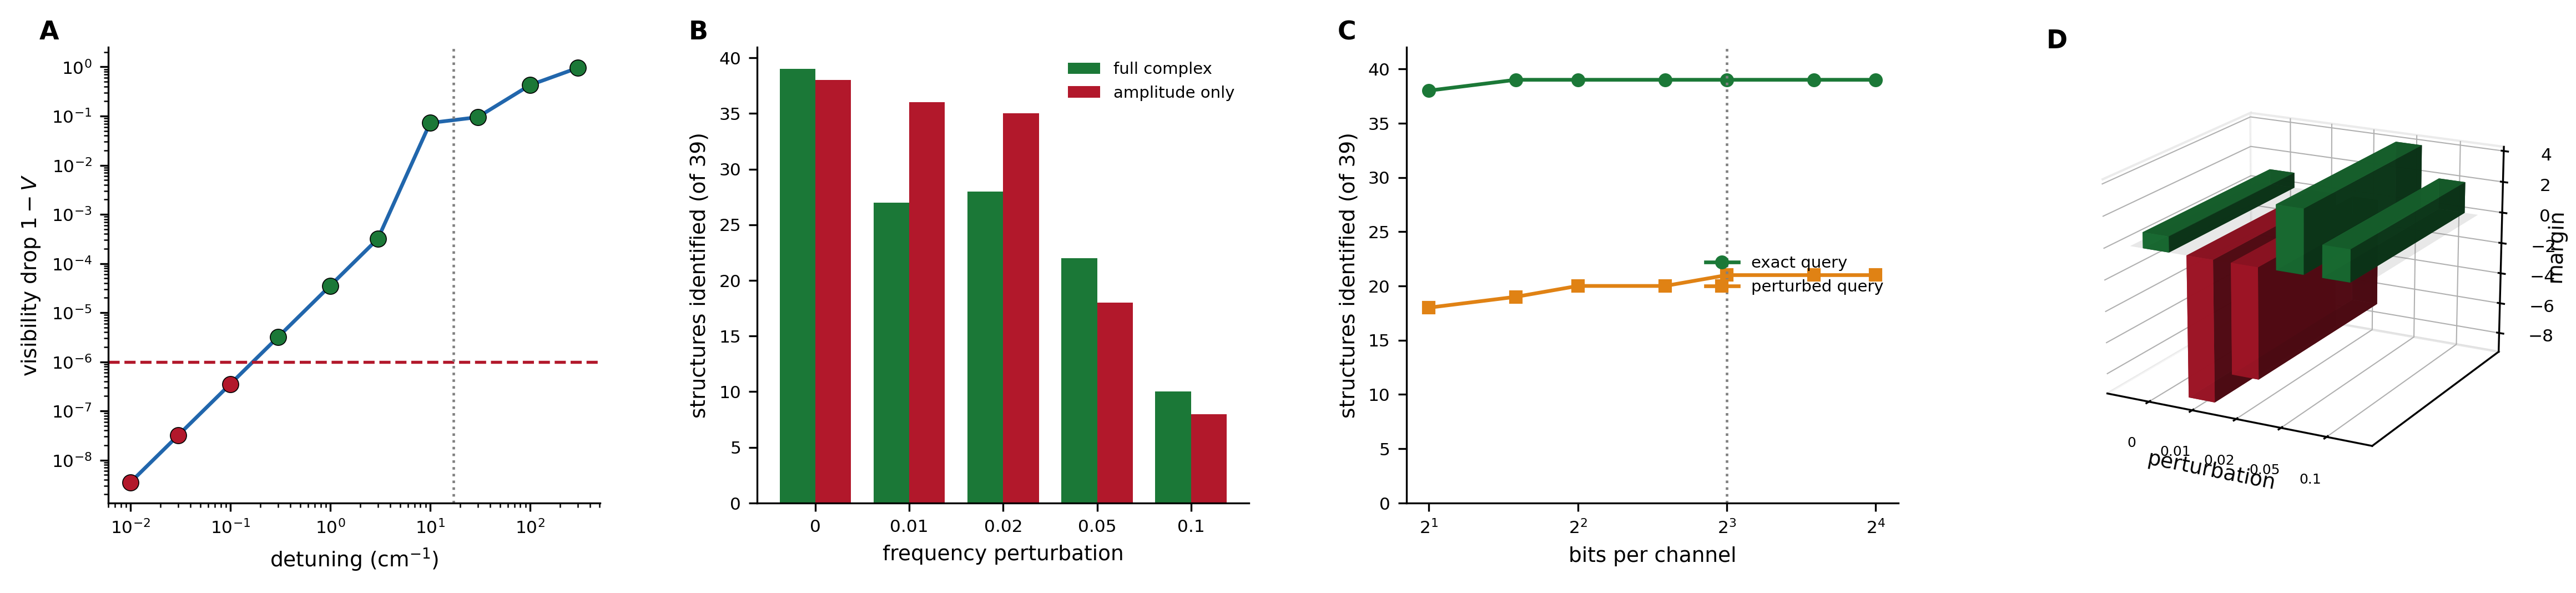
\includegraphics[width=\textwidth]{figures/panel_04_limits.png}
    \caption{\textbf{Three limits: the floor is declared rather than
    derived, the phase term is fragile, and display precision costs
    nothing.}
    (\textbf{A})~Visibility drop against detuning of one mode of a
    reference structure, on log--log axes, with the declared
    detectability threshold $10^{-6}$ (red dashed) and the grid cell
    width $17.19$~cm$^{-1}$ (grey dotted). Points are green where the
    drop exceeds the threshold and red where it does not. The smallest
    detectable detuning is $0.3$~cm$^{-1}$, a factor $0.017$ of the grid
    cell: the floor is not set by sampling, because the lobes are smooth
    and sampled rather than binned, so a sub-cell shift still moves every
    sample. What sets the floor is the threshold, which is an instrument
    parameter and must be declared (\Cref{rem:floorcriterion}).
    (\textbf{B})~The full complex comparison against an amplitude-only
    control, over increasing multiplicative frequency perturbation. The
    control \emph{beats} the full comparison at $1\%$ ($36$ against
    $27$) and $2\%$ ($35$ against $28$), and loses only from $5\%$
    onward. We had predicted the full comparison would dominate
    everywhere. The reading is that the accumulated phase of
    \Cref{eq:phase} is linear in mode frequency, so a small
    multiplicative perturbation of a high-frequency mode produces a large
    phase error and decoheres a comparison that amplitude alone would
    have got right.
    (\textbf{C})~Structures identified against bits per channel, for
    exact queries (green) and one fixed set of $5\%$ perturbed queries
    (orange), with $8$ bits marked. Both curves are flat from $8$ bits
    upward: $39/39$ and $21/39$ at $8$, $12$ and $16$ bits alike. Nothing
    measurable is lost by letting the displayed array be the compared
    array. An earlier version of this test drew fresh perturbations per
    depth and appeared to show low precision winning; that was a
    difference between query sets (\Cref{rem:rngartefact}).
    (\textbf{D})~The margin of panel~(\textbf{B}) --- full minus
    phaseless --- in three dimensions, with the zero plane drawn. Bars
    below the plane are perturbation levels at which the simpler control
    is better. The two red bars are the paper's clearest statement of
    where this construction should not be used: for spectra with
    sub-percent frequency uncertainty, an amplitude correlation is the
    better instrument.}
    \label{fig:limits}
\end{figure*}


% =====================================================================
\section{Relation to existing methods}
\label{sec:related}
% =====================================================================

\paragraph{Interferometric spectroscopy.} Acquiring a whole spectrum from
one superposed measurement is the basis of Fourier-transform
spectroscopy \citep{griffiths2007}, whose multiplex advantage
\citep{fellgett1949} is the same structural fact we exploit in
\Cref{thm:bulkid}. Our contribution is not the identity but the measured
limit on inverting it (\Cref{sec:capacity}); the multiplex advantage
concerns acquisition, and we find it does not transfer to pairwise
recovery.

\paragraph{Holography.} Recording relative phase against a reference and
reconstructing later \citep{gabor1948,goodman2005} is the mechanism our
stacking attempts to generalise to many objects at once. The failure in
\Cref{tab:capacity} is consistent with the classical requirement of a
distinct reference beam: with $n$ mutually interfering objects and no
reference, the cross-terms are not separable.

\paragraph{Phase retrieval.} Recovering phase from intensity is a
classical ill-posed inverse problem \citep{fienup1982,hadamard1902,
engl1996}. We do not solve it---our fields carry phase explicitly---but
\Cref{sec:control} shows the phase we carry is the fragile part, which is
consistent with why that literature is hard.

\paragraph{Spectral library search.} Library matching by similarity index
or contrast angle \citep{stein1994,wan2002,koo2011} solves the same task
as \Cref{sec:inversion} and is mature. We make no claim to outperform it;
\Cref{tab:control} shows a plain amplitude correlation beating our
comparison in the low-noise regime where library search operates.

\paragraph{Fingerprint similarity.} Structure-keyed and circular
fingerprints \citep{rogers2010,willett1998,riniker2013} compare extracted
features. The construction here differs in removing the comparison
function rather than choosing one, but this is an architectural
difference and we have not shown it to be an advantage on any task.

\paragraph{Molecular visualisation.} Established viewers
\citep{humphrey1996,pettersen2004,rego2015} render a structure computed
elsewhere. \Cref{sec:display} is the measurement relevant to whether
rendering and comparison can share one array; it says the precision is
sufficient, which is a necessary and not a sufficient condition for the
architectural claim.

% =====================================================================
\section{Limitations}
\label{sec:limits}
% =====================================================================

\begin{enumerate}[label=\textbf{L\arabic*.},leftmargin=2.8em,itemsep=4pt]

\item \textbf{Bulk comparison does not work.} \Cref{tab:capacity} is a
refutation, not a caveat. The scaling story---one superposition, all
pairs---is false operationally, and any use of this construction must
compare pairwise.

\item \textbf{The phase is fragile.} A phaseless control beats the full
comparison below $5\%$ frequency perturbation (\Cref{tab:control}).
In the low-noise regime the construction is worse than a simpler
alternative.

\item \textbf{Addressing resolves $69.2\%$.} Twelve of thirty-nine
structures share a cell at full depth, so the address is a screen and
the interference ranking is doing the identification work.

\item \textbf{The floor is declared, not derived.} The detectability
threshold $10^{-6}$ is an input. A different threshold gives a different
floor, and nothing in the construction determines it.

\item \textbf{The coordinate map is assumed.} \Cref{def:coords} takes
$\kappa$ as given. Every result is conditional on it, and we neither
derive nor test it.

\item \textbf{Isospectral structures are indistinguishable.} Two
structures with the same spectrum have the same field and visibility $1$,
so the instrument cannot separate them---by construction, not by
failure.

\item \textbf{One dimension, small set.} $G=256$ on a line, $39$ small
molecules assembled by others for another purpose. A corpus not chosen
for this test is weak evidence for anything beyond it
\citep{ioannidis2005}.

\item \textbf{No timing.} Every cost statement here is a count of
operations. No wall-clock measurement was made, and none should be
inferred.
\end{enumerate}

% =====================================================================
\section{Conclusion}
\label{sec:conclusion}
% =====================================================================

We asked what an instrument would be if run backwards---given a measured
value, return the structure---and built one. The construction realises
each structure as a complex field and compares two structures by adding
their fields, so that the relational content is the cross-term of a
superposition rather than the output of a similarity function.

Three things work. Self-comparison is exactly $1$ for all $39$ reference
structures, by Cauchy--Schwarz rather than by assumption, which repairs a
specification whose pointwise form attains only $0.528$ and requires an
unstated condition on phase. Inversion succeeds $39/39$: presented with a
spectrum, the instrument ranks the generating structure first. And
quantising the field to $8$ bits per channel---an ordinary
framebuffer---changes nothing, giving the same $39/39$ and $21/39$ as
$16$ bits, so the displayed array and the compared array can be the same
object.

One thing does not work, and it is the one the whole approach seemed to
promise. Superposition is linear, so a stack of $n$ structures contains
all $\binom{n}{2}$ cross-terms, and we confirmed that identity to a
relative residual of $0$ over $66$ pairs from a single addition. But the
cross-term bases are strongly non-orthogonal, and demodulation recovers
nothing: correlation with true pairwise visibility is $0.452$ at four
structures, negative from eight, with $17.5\%$ of projections diverging
at thirty-nine. The information is present and unreachable. Bulk
comparison at $O(1)$ in corpus size is refuted.

Two further results narrow the claim rather than support it. The phase
term that carries the coordinate information is fragile: below $5\%$
frequency perturbation a plain amplitude correlation identifies more
structures than the full complex comparison does. And the address route
resolves only $27$ of $39$ uniquely, so it is a screen and not an
identification.

What survives is narrower than what we set out to build, and we think it
is the more useful statement: comparison by superposition is exact,
display-precision-cheap, and strictly pairwise.

\section*{Reproducibility}

The experiment source records its expectations before the measured values
and writes every reported quantity to a JSON results file. Retained in
the source with their status marked are the vacuous floor criterion of
\Cref{rem:floorcriterion}, the undefined single-pair correlation of
\Cref{rem:n2}, the non-discriminating zero-perturbation control row of
\Cref{rem:controlhonest}, and the fresh-draw quantisation artefact of
\Cref{rem:rngartefact}, and the coordinate-rounding artefact of
\Cref{rem:rounding}. The only stochastic component is the frequency
perturbation, which seeds explicitly and is drawn once and reused across
bit depths. Numerical work uses double-precision arithmetic
\citep{ieee754,harris2020}.

\bibliographystyle{plainnat}
\bibliography{references}

\end{document}
